\chapter{Sensitivity of the Model}

A sensitivity analysis considers the extent to which uncertainty in model inputs influences model 
output.  For a sensitivity analysis, this uncertainty includes not only that inherent in the input of 
data for specific scenarios by the model user, but also uncertainty in empirical data or numerical 
parameters in the model such as the time step size used by the model to obtain a solution. 

Among the purposes for conducting a sensitivity analysis are to determine 
\begin{itemize}
\item the important variables in the models, 
\item the computationally valid range of values for each input variable, and 
\item the sensitivity of output variables to variations in input data. 
\end{itemize}

Conducting a sensitivity analysis of a complex model is not a simple task and it will differ 
depending on the application. CFAST typically requires the user to provide numerous input 
parameters that describe the building geometry, compartment connections, construction 
materials, and description of one or more fires. 

Iman and Helton \cite{Iman:1988} studied the sensitivity of complex computer models developed to simulate the risk of severe nuclear accidents which may include fire and other risks. Consistent with the 
work of Iman and Helton \cite{Iman:1988}, ASTM E1355 \cite{ASTM:E1355} provides overall guidance on typical areas of evaluation of the sensitivity of deterministic fire models.  These areas may involve one or more of the following techniques: finite difference or direct analysis methods that provide an explicit solution of the sensitivity equations associated with the governing equations of the model, 
factorial design or Latin hypercube sampling studies that investigate the effect of varying the 
input parameters and consequential interactions between parameters that may be deemed 
important, and global or response surface methods that investigate the overall behavior of model 
outputs for a desired range of inputs. 

This chapter provides a review of the sensitivity studies that have been conducted using CFAST 
with an emphasis on uncertainty in the input. Other sensitivity investigations of CFAST are also 
available \cite{Peacock:1988a, Beard:1992, Notarianni:2000}. 

\section{Factorial Design Studies}

Khoudja [\cite{Khoudja:1988} has studied the sensitivity of an early version of the FAST [2] (predecessor to CFAST) model with a fractional factorial design involving two levels of 16 different input 
parameters. The statistical design, taken from the texts by Box and Hunter \cite{Box:1978}, and Daniel \cite{Daniel:1976} reduced the necessary model runs from more than 65 000 to 256 by studying the interactions of input parameters simultaneously. The choice of values for each input parameter represented a range for each parameter. The analysis of the FAST model showed sensitivity to heat loss to the compartment walls and to the number of compartments in the simulation. Without the inclusion 
of surface thermophysical properties, this model treats surfaces as adiabatic for conductive heat 
transfer. Thus, consistent sensitivity should be expected. Sensitivity to changes in thermal 
properties of the surfaces were not explored. 

Walker \cite{Walker:1997} discussed the uncertainties in components of zone models and showed how 
uncertainty within user-supplied data affects the results of calculations using CFAST as an 
example. The study systematically varied inputs related to the fire (heat release rate, heat of 
combustion, mass loss rate, radiative fraction, and species yields) and compartment geometry 
(vent size and ceiling height) ranging from  $\pm$ 1 \% to $\pm$ 20 \% of base values for a one- 
compartment scenario. Heat release rate and ceiling height are seen to be the dominant input 
variables in the simulations. Upper layer temperature changed $\pm$ 10 \% for a $\pm$ 10 \% change in 
heat release rate. Typical variation of $\pm$ 10 s in time to untenable conditions for a 20 \% variation 
in the inputs was noted for the scenarios studied. 

Peacock et al. \cite{Peacock:1988a} studied the sensitivity of CFAST for a range of input parameters. They used simple factorial designs for model inputs deemed important to investigate local behavior of 
important model outputs along with response surface methods to evaluate overall model 
behavior. Results of the parametric investigations are discussed below and the application of 
response surface methods is summarized in section 5.2. Both are discussed in more detail in 
reference \cite{Peacock:1988a}.

\subsection{Model Inputs and Outputs}

Most studies of modeling related to fire hazard and fire reconstruction present a consistent set of 
variables of interest to the model user \cite{Emmons:1988, Duong:1990, Beard:1992, NRCNUREG1824Overview} : upper and lower gas layer temperatures, gas species concentrations, and layer interface position. Other variables of interest include 

\begin{itemize}
\item mass pyrolysis and heat release rate, 
\item room pressure, and 
\item vent flow. 
\end{itemize}

Although there are certainly other comparisons of interest, these will provide evidence of the 
sensitivity of the model to most model inputs.  Tables 4 and 5 show typical inputs and outputs 
for the CFAST model.

\begin{table}
\begin{center}
\caption{Typical Inputs for a Two-Zone Fire Model}
\label{tab:Two_Zone_Inputs}
\begin{tabular}{| p{1.5in} | p{4.5in} |}
\hline
Ambient Conditions & Inside temperature and pressure.

Outside temperature and pressure.

Wind speed.

Relative humidity \\  \hline \hline
Building Geometry & Compartment width, depth, height, and surface material properties (conductivity, heat capacity, density, thickness).

Horizontal Flow Vents: Height of soffit above floor, height of sill above floor, width of vent, angle of wind to vent, time history of vent openings and closings.

Vertical Flow Vents: Area of vent, shape of vent.

Mechanical Ventilation, Orientation of vent, Center height of vent, area of vent, length of ducts, diameter of ducts, duct roughness, duct flow coefficients, fan flow characteristics. \\ \hline \hline
Fire Specification & 	Fire room, X, Y, Z position in room, fire area.
Fire Chemistry: Molar Weight, Lower oxygen limit, heat of combustion, initial fuel temperature, gaseous ignition temperature, radiative fraction.
Fire History: Mass loss rate, heat release rate, species yields for HCN, HCl, H/C, O\subscript{2}/C, C/CO\subscript{2}, CO/CO\subscript{2}. \\ \hline
\end{tabular}
\end{center}
\end{table}

\begin{table}
\begin{center}
\caption{Typical Outputs for a Two-Zone Fire Model}
\label{tab:Two_Zone_Outputs}
\begin{tabular}{| p{1.5in} | p{4.5in} |}
\hline
Environment & for each compartment: Compartment pressure and layer interface height.
 
for each layer and compartment: Temperature, layer mass density, layer volume, heat release rate, gas concentrations (N2, O2, CO2, CO, H2O, HCl, HCN, soot optical density), radiative heat into layer, convective heat into layer, heat release rate in layer.
 
for each vent and layer: Mass flow, entrainment, vent jet fire.

for each fire: Heat release rate of fire, mass flow from plume to upper layer, plume entrainment, pyrolysis rate of fire.

for each compartment surface: Surface temperatures. \\  \hline \hline
Tenability & Temperature.
  
  Fractional Effective Dose (FED). \\ \hline
\end{tabular}
\end{center}
\end{table}

Consider the following fire scenario: The building geometry (figure \ref{fig:Sensitivity_BaseCase}) includes four rooms on two floors with horizontal, vertical, and mechanical vents connecting the rooms and venting to the outdoors. The fire source in one of the rooms on the lower floor is a medium growth rate t-squared fire \cite{NFPA72:2003} chosen to simulate a mattress fire \cite{Babrauskas:1985}.

\begin{figure}[t]
\begin{center}
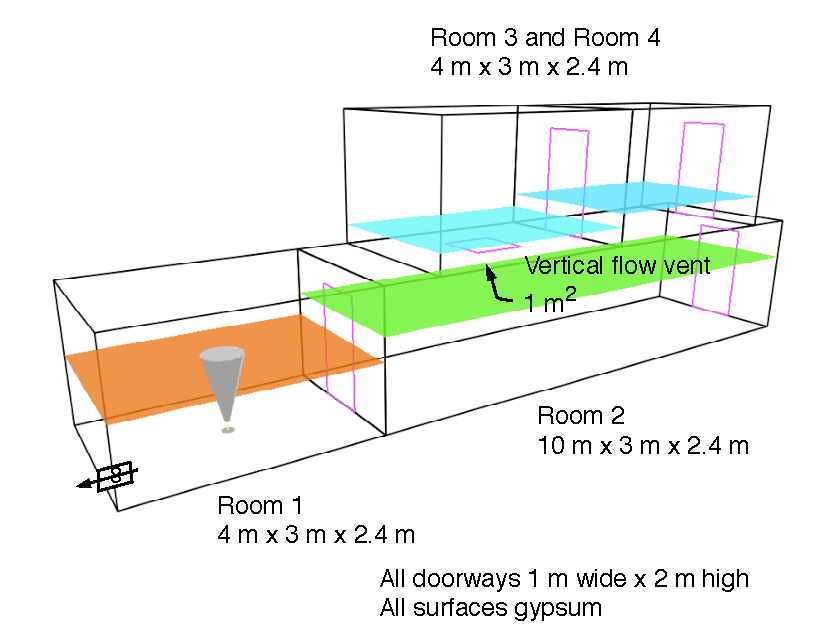
\includegraphics[width=4.5in]{FIGURES/Sensitivity/SensitivitySample}\\
\end{center}
\caption{Building Geometry for base case scenario.}
 \label{fig:Sensitivity_BaseCase}
\end{figure}

\subsubsection{Sensitivity to Small Changes in Model Inputs}

To investigate the sensitivity of the model, a number of simulations were conducted varying the input parameters about the base scenario discussed in the previous section. Both small ($\pm$10 \%) and larger (up to an order of magnitude) variations for selected inputs were studied. Varying most of the inputs by small amounts had little effect on the model outputs. Figure \ref{fig:Sensitivity_Volume10Percent} presents an example of the time dependent sensitivity of several outputs to a 10 \% change in room volume for the fire compartment in the scenario described above. For example, the pair of dotted-line curves labeled �Upper Layer Volume� were created by comparing the base case scenario with a scenario whose compartment volume was increased and decreased by 10 \%. The resulting curves presented on the graph are the relative difference between the variant cases and the base case defined by (Variant value - Base value) / Base value for each time point. The graph shows that temperature and pressure are insensitive to changes in the volume of the fire room since a 10 \% change in room volume led to smaller relative changes in layer temperature and room pressure for all times. Upper layer volume can be considered neutrally sensitive (a 10 \% change in room volume led to about a 10 \% change in layer volume). Further, this implies that there is negligible effect on the average layer interface height. This is consistent with both experimental observations in open compartment room fires  and analytical solutions for single compartment steady-state fires . For transient conditions early in the fire or when the fire burns out (illustrated in the figure at 300 s when the gas burner fire heat release rate goes to zero) higher uncertainties are noted.  While these are transient effects, the early phases of the fire, in particular, may be important in calculating tenability for occupants during egress. While an uncertainty in the compartment volumes results in an equivalent uncertainty in calculated outputs, accurate specification of compartment dimensions within 5 \% is often easily obtained.

\begin{figure}
\begin{center}
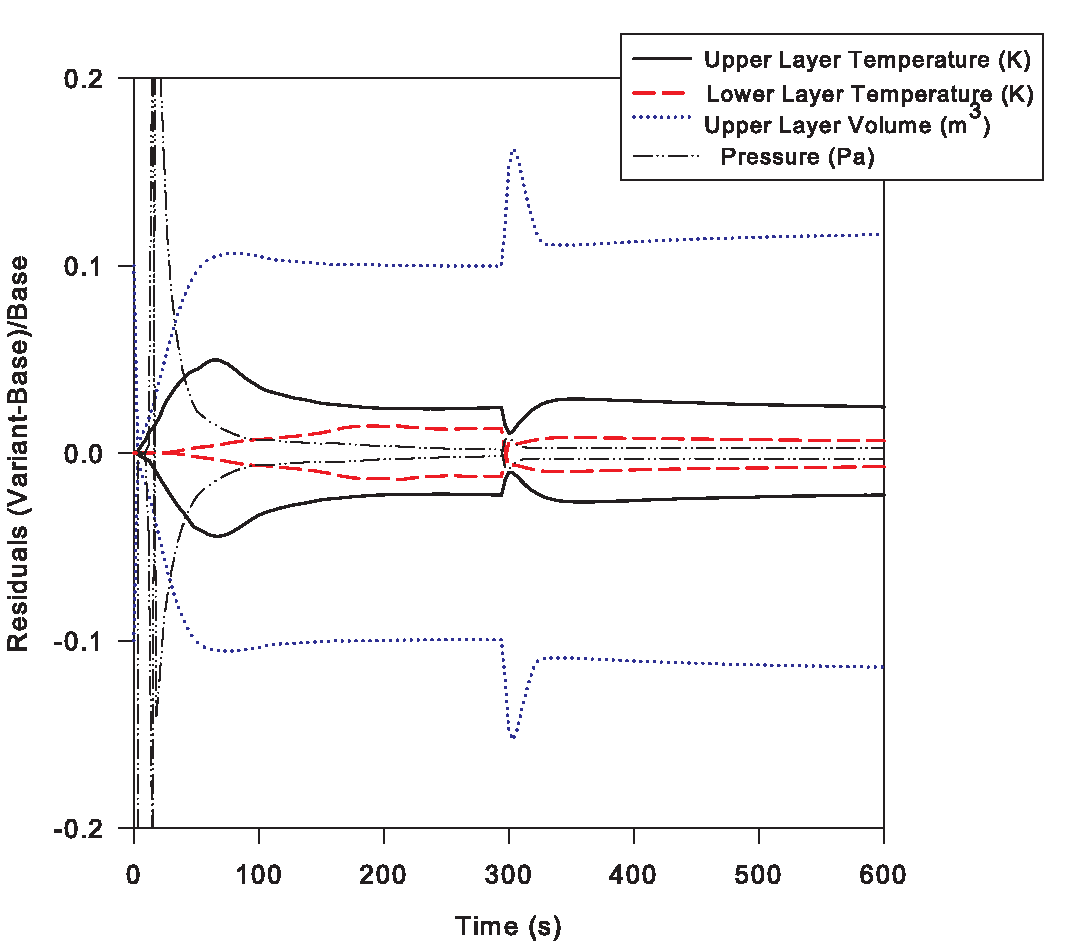
\includegraphics[width=4in]{FIGURES/Sensitivity/Volume_Sensitivity}\\
\end{center}
\caption{An example of time dependent sensitivity of fire model outputs to a 10 \% change in room volume for a single room fire scenario.}
 \label{fig:Sensitivity_Volume10Percent}
\end{figure}

In addition, figure \ref{fig:Sensitivity_Volume10Percent} shows a somewhat constant relative difference for the changes as a function of time. As suggested by Iman and Helton [\cite{Iman:1988}, an average relative difference could thus be used to characterize the model sensitivity for comparing individual inputs and outputs.

\subsection{Sensitivity to Larger Changes in Model Inputs}

To investigate the effects of much larger changes in the inputs, a series of simulations was conducted where the inputs were varied from 10 \% to 400 \% of base values. Simulations changing the heat release rate inputs from the base peak heat release rate of 750 kW are shown in figure \ref{fig:Sensitivity_VolumeFamilies}. 

\begin{figure}
\begin{center}
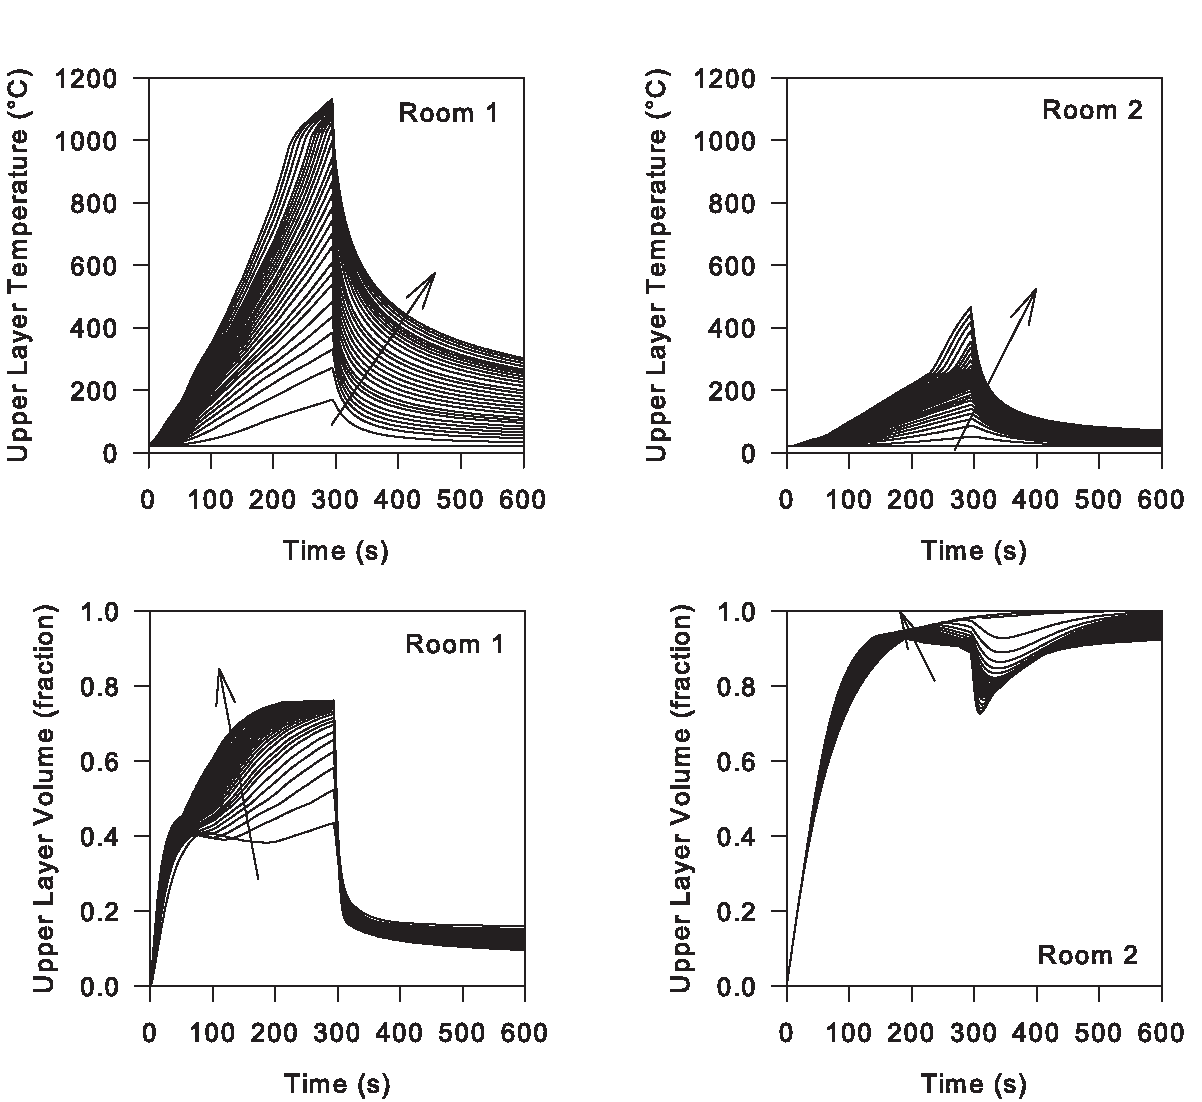
\includegraphics[width=6in]{FIGURES/Sensitivity/Volume_Families}\\
\end{center}
\caption{Layer temperatures and volumes in several rooms resulting from variation in heat release rate for a four-room growing fire scenario.}
 \label{fig:Sensitivity_VolumeFamilies}
\end{figure}

Each set appears as families of curves with similar functional forms. This indicates that the heat release rate has a monotonic effect on the layer temperatures, with not as clear an effect on upper layer volume due to compartment filling and flow between compartments. Like the sensitivity to compartment volume in the previous section, changing the heat release rate by a factor of two results in a factor of two change in the upper layer temperature.  Thus, in absolute terms, heat release rate and compartment volume are equally sensitive.  However, compartment volume is easily determined accurately while heat release rate is typically estimated with far less accuracy and may be uncertain to within an order of magnitude or larger. 

In the majority of fire cases, the most crucial question that can be asked by the person responsible for fire protection is: �How big is the fire?� Put in quantitative terms, this translates to: �What is the heat release rate of this fire?� Recently the National Institute of Standards and Technology (NIST) examined the pivotal nature of heat release rate measurements in detail \cite{Babrauskas:1992}. Not only is heat release rate seen as the key indicator of real-scale fire performance of a material or construction, heat release rate is, in fact, the single most important variable in characterizing the �flammability� of products and their consequent fire hazard.  Much of the remainder of this paper focuses on heat release rate as an example for examining sensitivity analysis.

\section{Response Surface Studies}

A next step beyond the simple plots presented in figure \ref{fig:Sensitivity_VolumeFamilies} is a cross-plot of outputs of interest against heat release rate. Figure \ref{fig:Sensitivity_ULTvsHRR} presents plots of the upper layer temperature (presented in figure \ref{fig:Sensitivity_VolumeFamilies}) plotted against the heat release rate for all the simulations. The temperature curves for upper layer temperature in all four rooms (figure \ref{fig:Sensitivity_ULTvsHRR}) show a strong functional dependence on heat release rate. Even for the wide variation in inputs, the heat release rate provides a simple predictor of the temperature in the rooms. In addition, this relationship allows calculation of the sensitivity of the temperature outputs to the heat release rate inputs as a simple slope of the resulting correlation between heat release rate and temperature. 

\begin{figure}
\begin{center}
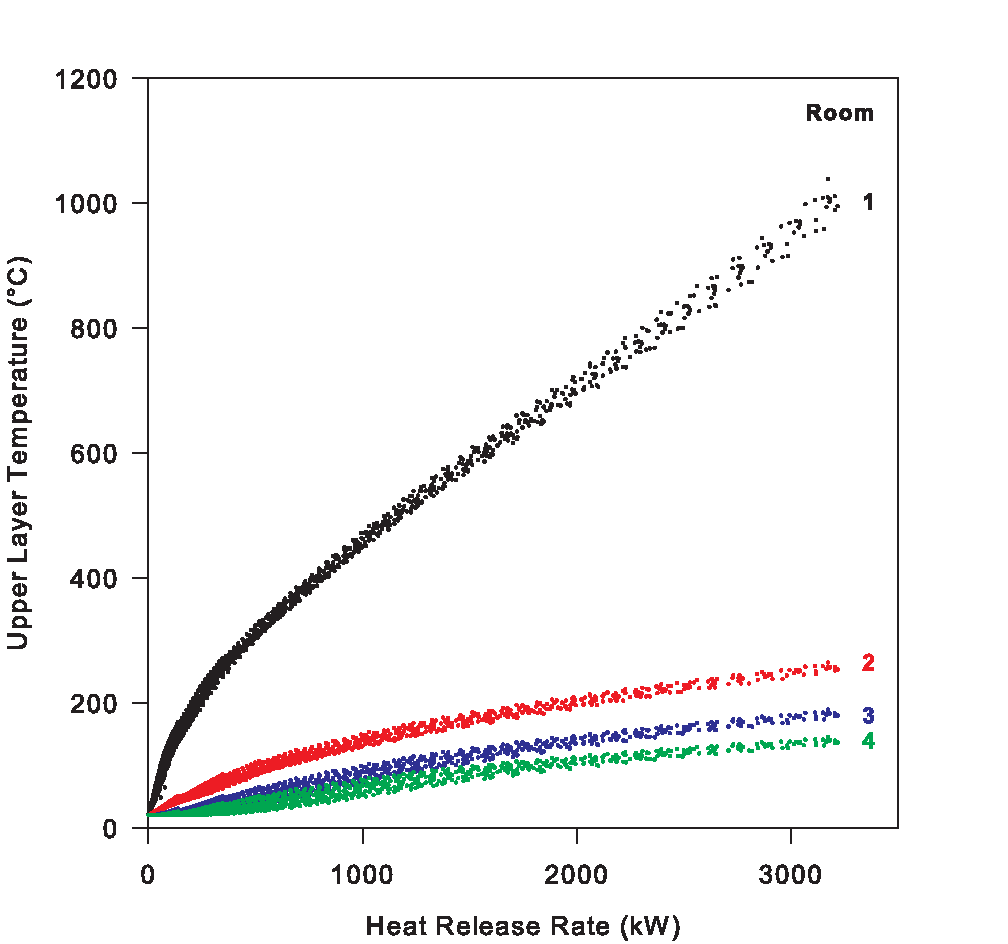
\includegraphics[width=4in]{FIGURES/Sensitivity/ULTvsHRR}\\
\end{center}
\caption{Comparison of the time dependent heat release rate and layer temperatures in several rooms for a four-room growing fire scenario.}
 \label{fig:Sensitivity_ULTvsHRR}
\end{figure}

Figure \ref{fig:TempSensitivity}, simply a plot of the slope of the regression curves in figure \ref{fig:Sensitivity_ULTvsHRR}, shows this sensitivity, $\partial (T)/\partial (heat release rate)$, for the four-room scenarios studied and represents all time points in all he simulations in which the peak heat release rate was varied from 0.1 to 4.0 times the base value. Except for relatively low heat release rate, the upper layer temperature sensitivity is less than 1 K/kW and usually below 0.2~K/kW.  Not surprisingly, the layer that the fire feeds directly is  most sensitive to changes.  The lower layer in the fire room and all layers in other rooms have sensitivities less than 0.2 K/kW. This implies, for example, that if the heat release rate for a 1 MW fire is known to within 100 kW, the resulting uncertainty in the calculation of upper layer temperature in the fire room is about $\pm$ 30 K.

\begin{figure}
\begin{center}
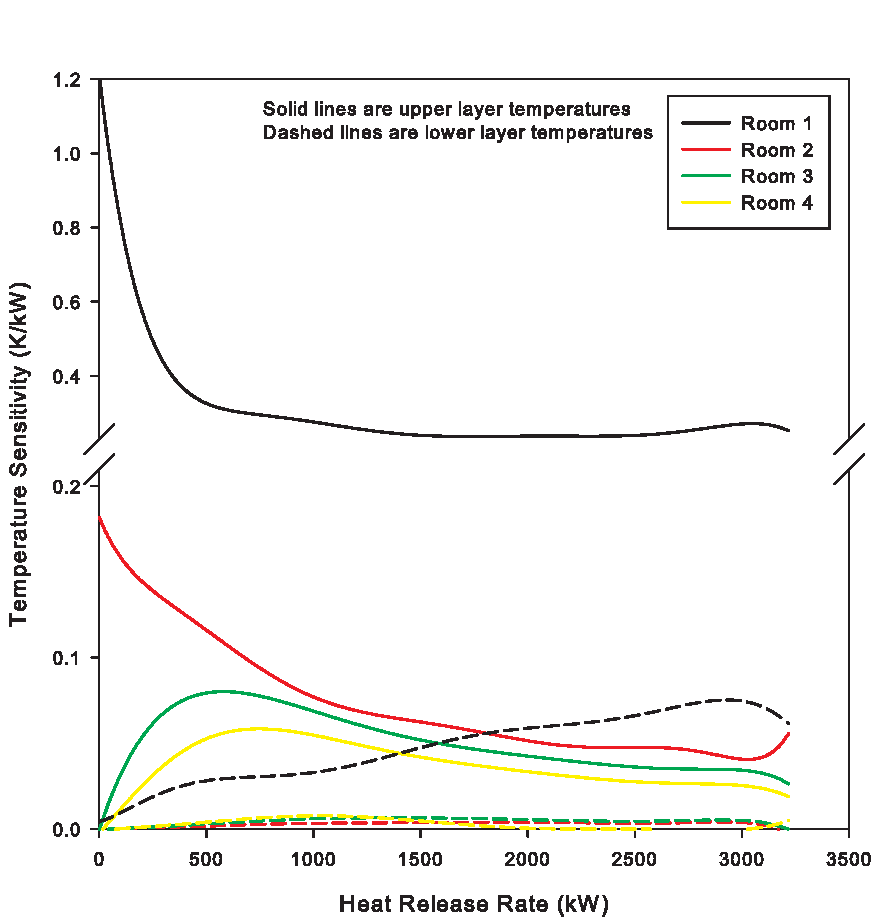
\includegraphics[width=4in]{FIGURES/Sensitivity/TempSensitivity}\\
\end{center}
\caption{Sensitivity of temperature to heat release rate for a four-room growing fire scenario.}
 \label{fig:TempSensitivity}
\end{figure}

For upper layer volumes (figure \ref{fig:VolumeSensitivity}) of both rooms 1 and 2, it is again a simple correlation between heat release rate and volume fraction (upper layer volume expressed as a fraction of the total room volume). The shaded gray area on the graph shows the locus of all individual time point values of temperature and volume in the four compartments of the simulation. The correlations for the upper layer volumes of room 1 and room 2 could also be differentiated as was done for the temperature correlations to obtain sensitivities for the upper layer volume. For rooms 3 and 4, the relationship is not as clear. The flow into the layers of these rooms is more complicated than for rooms 1 and 2, resulting from flow from the first floor through a vent in the floor of room 3 and from a vent to the outside in room 4. However, even these rooms approach a constant value for higher heat release rate values, implying near zero sensitivity for high heat release rate.

\begin{figure}
\begin{center}
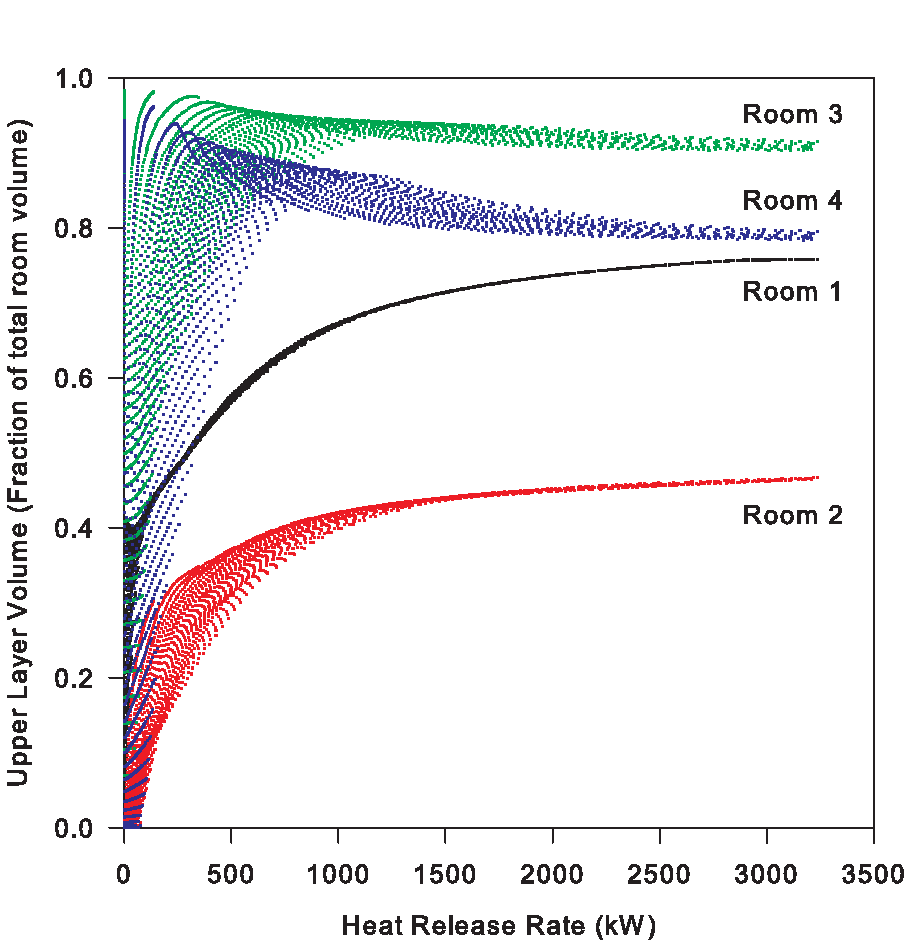
\includegraphics[width=4in]{FIGURES/Sensitivity/VolumeSensitivity}\\
\end{center}
\caption{Sensitivity of temperature to heat release rate for a four-room growing fire scenario.}
 \label{fig:VolumeSensitivity}
\end{figure}

Figure \ref{fig:Sensitivity3D} presents the effect of both peak heat release rate and vent opening (in the fire room) on the peak upper layer temperature. In this figure, actual model calculations, normalized to the base scenario values are indicated by circles overlaid on a surface grid generated by a spline interpolation between the data points. At high heat release rate and small vent openings, the fire becomes oxygen limited and the temperature trails off accordingly, but for the most part, the behavior of the model is monotonic in nature. Although more laborious, the approaches used to calculate sensitivities for single variable dependencies illustrated earlier are thus equally applicable to multivariate analyses.

From the surface, it is clear that heat release rate has more of an effect on the peak temperature than does the vent width. Until the fire becomes oxygen limited, the trends evident in the surface are consistent with expectations � temperature goes up with rising heat release rate and down with rising vent width. The effects are not, of course, linear with either heat release rate or vent opening. Plume theory and typically used algorithms for estimating upper layer temperature in a single room with a fire  suggest that the dependence is on the order of $Q_f^{2/3}$ for heat release rate and $A \sqrt{h}$ for the vent opening where $A$ is the area of the vent and $h$ is the height of the vent. Although these correlations are based on a simple analysis of a single room fire, the dependence suggested is similar to that illustrated in figure \ref{fig:Sensitivity3D}.

\begin{figure}
\begin{center}
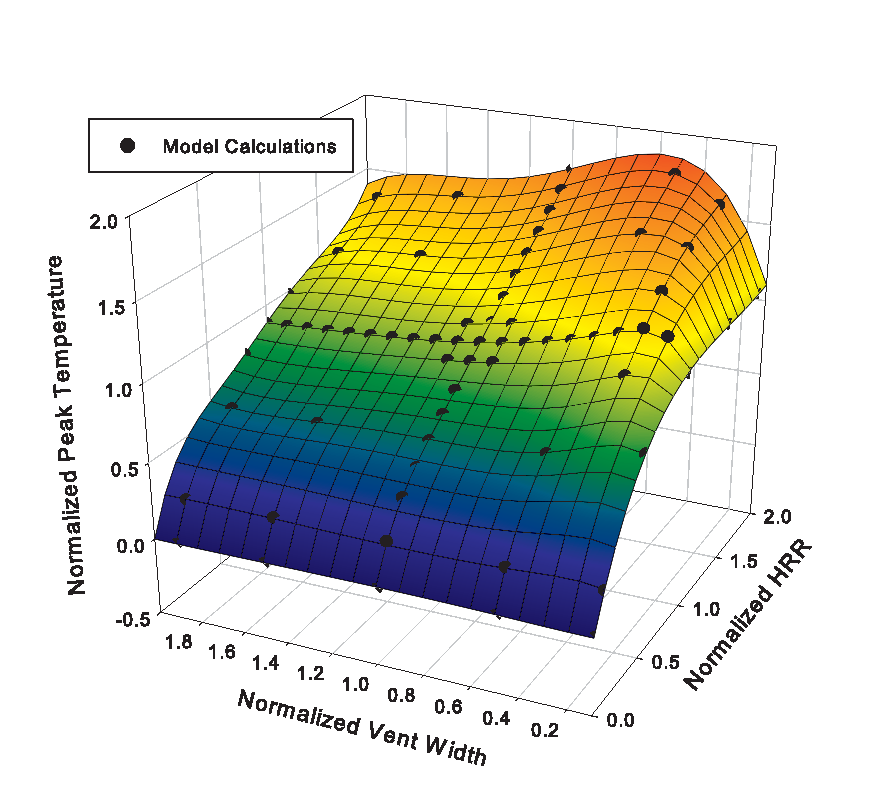
\includegraphics[width=4in]{FIGURES/Sensitivity/Sensitivity3D}\\
\end{center}
\caption{Sensitivity of temperature to heat release rate for a four-room growing fire scenario.}
 \label{fig:Sensitivity3D}
\end{figure}

\section{Latin Hypercube Sampling Studies}

Notarianni \cite{Notarianni:2000} developed an iterative methodology for the treatment of uncertainty in fire-safety engineering calculations to identify important model parameters for detailed study of uncertainty.  She defines a nine-step process to identify crucial model inputs and parameters, select sampling methods appropriate for the important parameters, and evaluate the sensitivity of the model to chosen outcomes. Both factorial designs and Latin hypercube sampling are included in a case study involving the CFAST model.  In a performance-based design of a 16 story residential structure, the impact of model uncertainty on a chosen design and inclusion of residential sprinklers in the design would effect the resulting safety of the design.  For a seven-compartment scenario representing one living unit in the structure, distributions of input variables based on Latin hypercube sampling of selected ranges of the inputs were developed and used as input for a series of 500 CFAST simulations for the scenario. The results of the calculations are presented in a series of cumulative distribution functions which show the probability that a chosen criterion of the design is exceeded within a given time. Depending on the evaluation criterion chosen, times to unacceptable designs varied by as little as 10 s to as much as 470 s. To determine important input variables, Notarianni used a multivariate correlation of the input and output variables to determine statistical significance at a 95 \% confidence level. Input variables deemed important in the analysis included fire-related inputs (growth rate, heat of combustion, position of the base of the fire, and generation rates of products of combustion) and door opening sizes.  Other inputs were determined to be less important.

\section{Summary}

Many of the outputs of the CFAST model are quite insensitive to uncertainty in the input parameters for a broad range of scenarios. Not surprisingly, heat release rate was consistently seen as the most important variable in a range of simulations.  Heat release rate and related variables such as heat of combustion or generation rates of products of combustion provide the driving force for fire-driven flows.  For CFAST, all of these are user inputs.  Thus, careful selection of these fire related variables are necessary for accurate predictions.  Other variables related to compartment geometry such as compartment height or vent sizes, while deemed important for the model outputs, are typically more easily defined for specific design scenarios than fire related inputs.  For some scenarios, such as typical building performance design, these vents may need to include the effects of leakage to insure accurate predictions. For other scenarios, such as shipboard use or nuclear power facilities, leakage (or lack thereof) may be easily defined and may not be an issue in the calculations.